\chapter{急性腹泻}

正常人大便次数差异较大,每日1~3次或每周2~3次不等,一般重量为150~200g/d,含水量60\%~80\%。腹泻(diarrhea)是指排便次数增加(如每日超过3次)、排粪量增加(超过200g/d)、粪质稀薄(含水量超过80\%)。如每日排粪量超过1000g者为严重腹泻。

急性腹泻的病程一般在3周之内,往往伴有肠痉挛所致的腹痛。

急性腹泻最常见的原因是细菌性食物中毒与肠道感染。急性腹泻在诊断与鉴别诊断方面须特别注意下列情况:

\section{【病史采集要点】}

\subsection{(一)起病情况}

起病急、病程短而腹泻次数频繁者,应考虑各种感染所引起的急性腹泻。应注意流行病学调查,是否是集体或家人在短期内先后发病。食物中毒泛指源于食物的暴发性流行病伴痢疾、水样泻或胃肠道以外的症状,可由于有毒食物(如毒蕈、毒鱼)本身或细菌污染所致,后者又称细菌性食物中毒。非感染性腹泻如食物过敏,往往在进食后几小时突觉脐周剧烈疼痛、水样泻2~3次自愈,可能由耐热的蛋白质过敏原引起。可伴有荨麻疹、血中嗜酸性粒细胞增多。甲亢危象时,可因自主神经功能的紊乱而发生急性腹泻,奔跑者腹泻则可能为促胃液素、胃动素、血管活性肠肽及前列腺素释放之故。

小儿夏秋季流行性腹泻,经多次大便培养未发现致病菌者,须注意病毒性肠炎。较长期接受广谱抗生素治疗的患者,突然发生腹泻,须考虑抗生素相关性腹泻及假膜性肠炎。

\subsection{(二)大便量及性质}

从粪便肉眼观察及病史等,可区别源于小肠或结肠的腹泻(表\ref{tab23-1})。

\begin{table}[htbp]
\centering
\caption{小肠性腹泻与结肠性腹泻的鉴别}
\label{tab23-1}
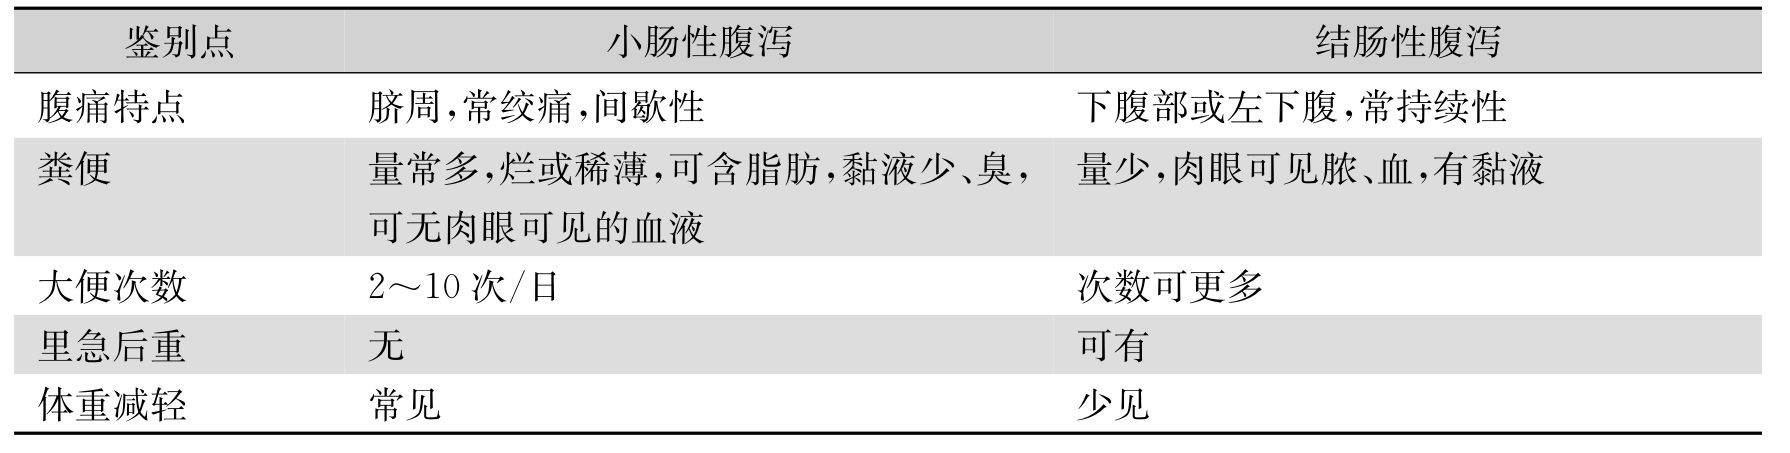
\includegraphics[width=5.95833in,height=1.5in]{./images/Image00124.jpg}
\end{table}

大便量>500ml/d多为分泌性腹泻。脓血便为渗出性腹泻。如脓血和大便不混,常是直肠或乙状结肠炎症。果酱样便见于阿米巴痢疾,蛋花样便见于假膜性肠炎,大便有油脂光泽、有泡沫为脂肪吸收障碍,大便恶臭为蛋白质消化吸收不良,酸臭糊状便为糖吸收障碍。

急性腹泻可分水样泻和痢疾样泻。水样泻时肠黏膜可无破坏、不含血或脓,可不伴里急后重,腹痛较轻。痢疾样泻表示肠黏膜有破坏,有脓血便,常伴里急后重与腹绞痛。两者可并存(表\ref{tab23-2})。水样泻常系细菌毒素如霍乱弧菌等的肠毒素引起,痢疾样泻可见于细菌性痢疾、阿米巴肠病、急性溃疡性结肠炎等。

\begin{table}[htbp]
\centering
\caption{水样泻、痢疾样泻和混合型的鉴别}
\label{tab23-2}
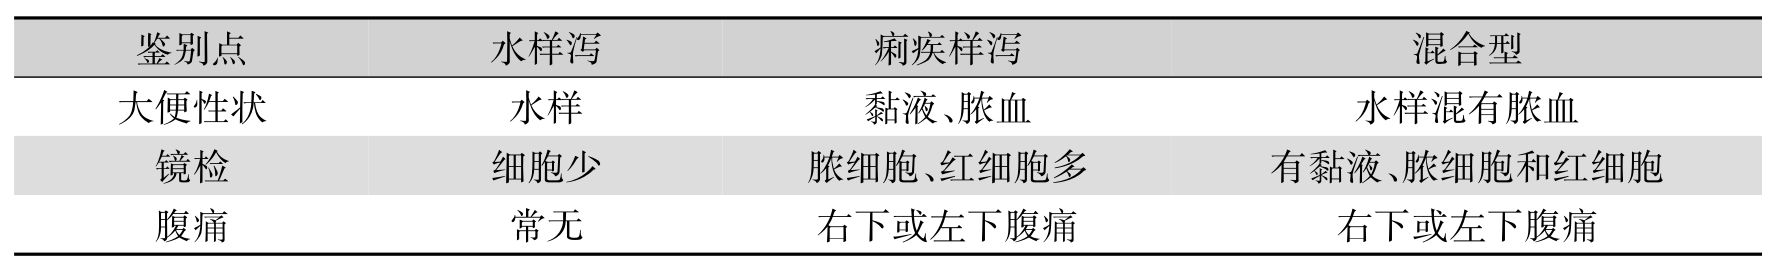
\includegraphics[width=5.91667in,height=0.89583in]{./images/Image00125.jpg}
\end{table}

\section{【体格检查重点】}

全身状况包括生命体征、营养状况、贫血、恶病质、淋巴结肿大、皮肤黄染、突眼等。腹部检查应注意有无腹胀、腹部肿块、压痛、肠鸣音、肠蠕动等,并常规行肛门指检。

\section{【实验室及器械检查】}

主要是粪便检查,包括外观、量、镜检细胞、原虫、虫卵、隐血试验、涂片查菌群及细菌和真菌培养,这些检查均可初步确定是否是炎症性或感染性腹泻。

细菌性食物中毒的粪便常呈糊样或水样,红、白细胞无或量少。脓血便伴里急后重者以急性细菌性痢疾可能性大,空肠弯曲菌性肠炎、耶尔森菌性肠炎、侵袭性大肠杆菌肠炎等也可有同样表现。带恶臭的血样便,应注意出血性坏死性肠炎、阿米巴肠病等。米泔水样便应考虑霍乱。

粪便镜检应尽量采用新鲜标本,对检查阿米巴原虫尤为重要。致病菌的培养应在疾病早期并在应用抗菌药物治疗之前进行,应选取粪便的脓血部分送检。血清凝集反应检测致病菌抗体有助于细菌性食物中毒和某些急性肠道感染的诊断。

急性腹泻患者一般不行结肠镜检查。对疑有假膜性肠炎者,可行结肠镜或直肠镜检查,可发现假膜。

图\ref{fig23-1}为急性腹泻诊断思路。

\begin{figure}[!htbp]
 \centering
 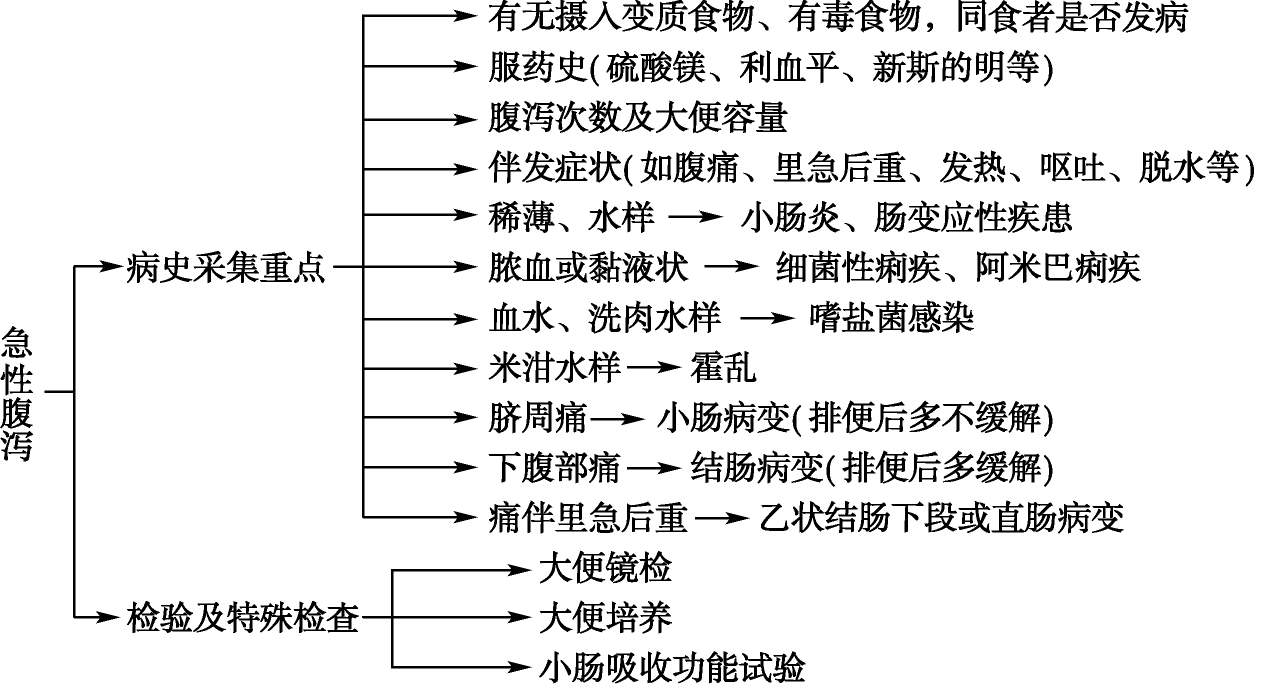
\includegraphics[width=4.44792in,height=2.44792in]{./images/Image00126.jpg}
 \captionsetup{justification=centering}
 \caption{急性腹泻诊断思路}
 \label{fig23-1}
  \end{figure} 

急性腹泻的常见病因见表\ref{tab23-3}。

\begin{table}[htbp]
\centering
\caption{引起急性腹泻的常见病因分类}
\label{tab23-3}
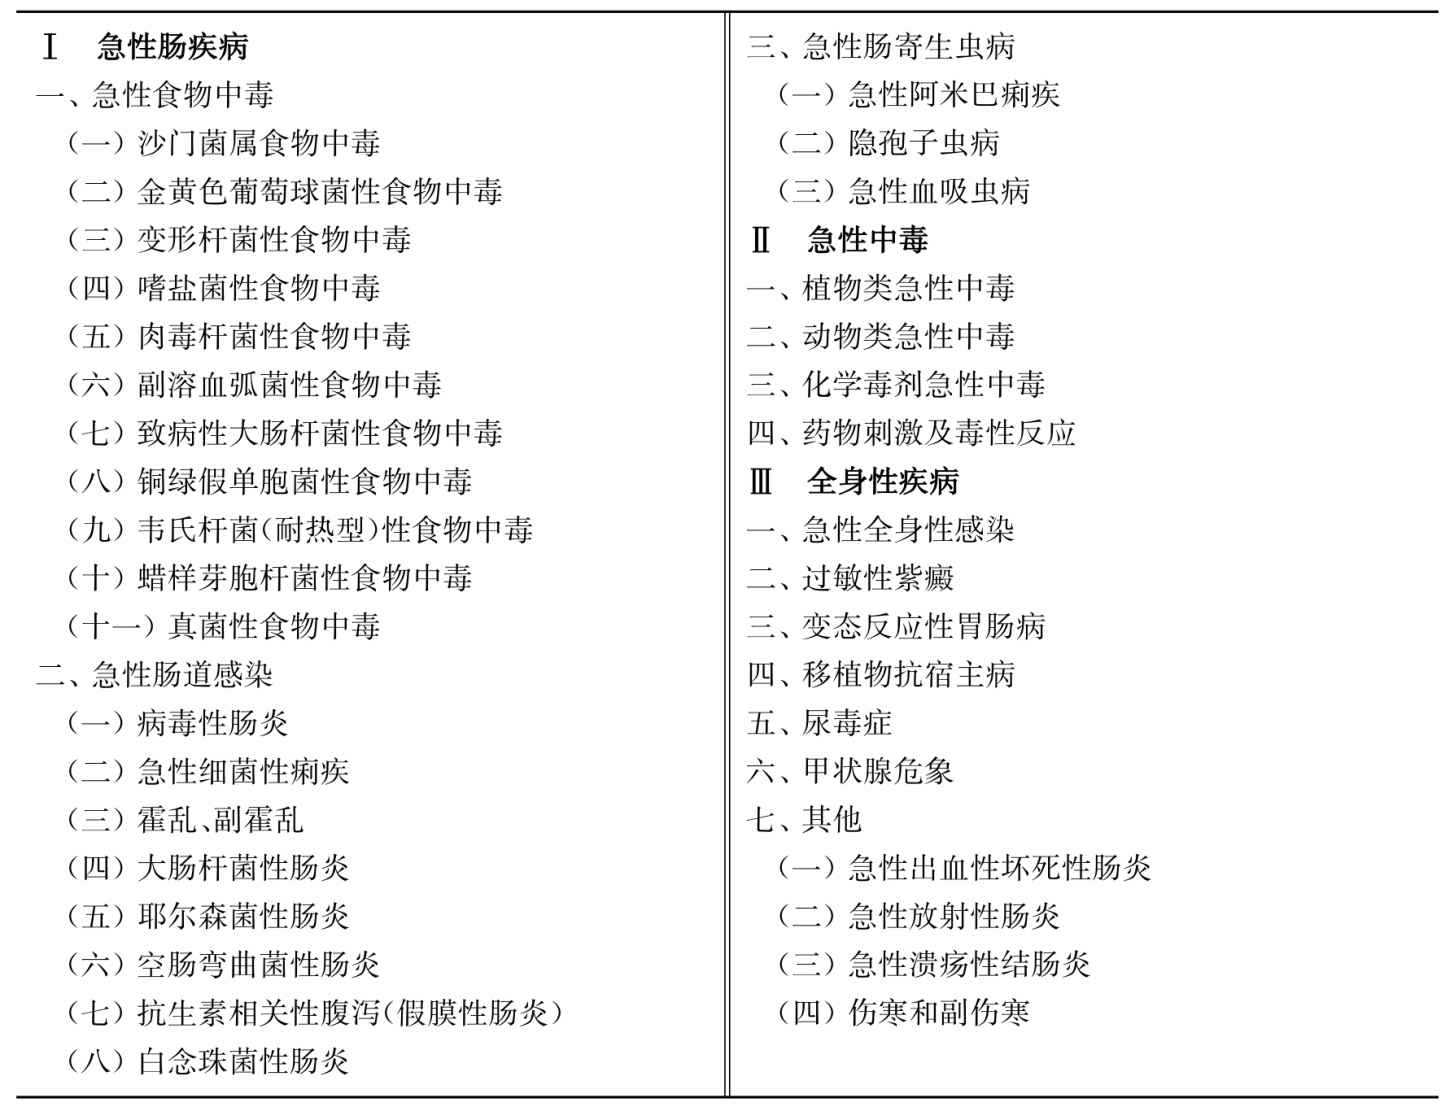
\includegraphics[width=5.94792in,height=4.58333in]{./images/Image00127.jpg}
\end{table}

\protect\hypertarget{text00183.html}{}{}

\section{73 急性肠疾病}

\subsection{73.1 急性细菌性食物中毒}

细菌性食物中毒是临床上最常见的一种急性(胃)肠炎。本病是由于进食被细菌或其毒素污染的食物所致的中毒性疾病,往往有同席多人或在同一单位中集体发病的流行病学特点,急性呕吐与腹泻常是主要的临床表现。

\subsubsection{一、沙门菌属性食物中毒}

沙门菌属性食物中毒是细菌性食物中毒的主要形式,常由于食物(肉类、蛋类、鱼类)污染而暴发大、小的流行。往往同席多人或在集体食堂中多人发病。致病菌以肠炎、鼠伤寒与猪霍乱沙门菌较为常见。沙门菌属所致的食物中毒,不但表现为急性胃肠炎,而且还有发热等全身性感染的症状,早期还可出现菌血症。伤寒及副伤寒亦属沙门菌属,见后详述。

潜伏期一般为8~24小时。起病急骤,常伴有恶寒、发热,但热度一般不甚高,同时出现腹绞痛、胀气、恶心、呕吐等症状。继而发生腹泻,一天数次至十几次或更多,如水样,深黄色或带绿色,有些恶臭。粪便中常混有未消化的食物及少量黏液,偶带脓血。当炎症蔓延至结肠下段时,可有里急后重。病程大多为2~4天,有时较长。

偶有呈霍乱样暴发性急性胃肠炎型者,患者呕吐与腹泻均剧烈,体温在病初时升高,后即下降,脉弱而速,可出现严重脱水、电解质紊乱、肌肉痉挛、尿少或尿闭,如抢救不及时,可于短期内因急性肾衰竭或周围循环衰竭而死亡,此型须与其他细菌性食物中毒、霍乱、副霍乱及急性菌痢相区别(表\ref{tab23-4})。残留食物、患者呕吐物与粪便培养沙门菌属阳性,早期血培养有时阳性,恢复期患者血清沙门菌凝集效价明显增高,有助于鉴别诊断。

\begin{longtable}{c}
 \caption{各种细菌性食物中毒、副霍乱、霍乱、急性菌痢的鉴别}
 \label{tab23-4}
 \endfirsthead
 \caption[]{各种细菌性食物中毒、副霍乱、霍乱、急性菌痢的鉴别}
 \endhead
 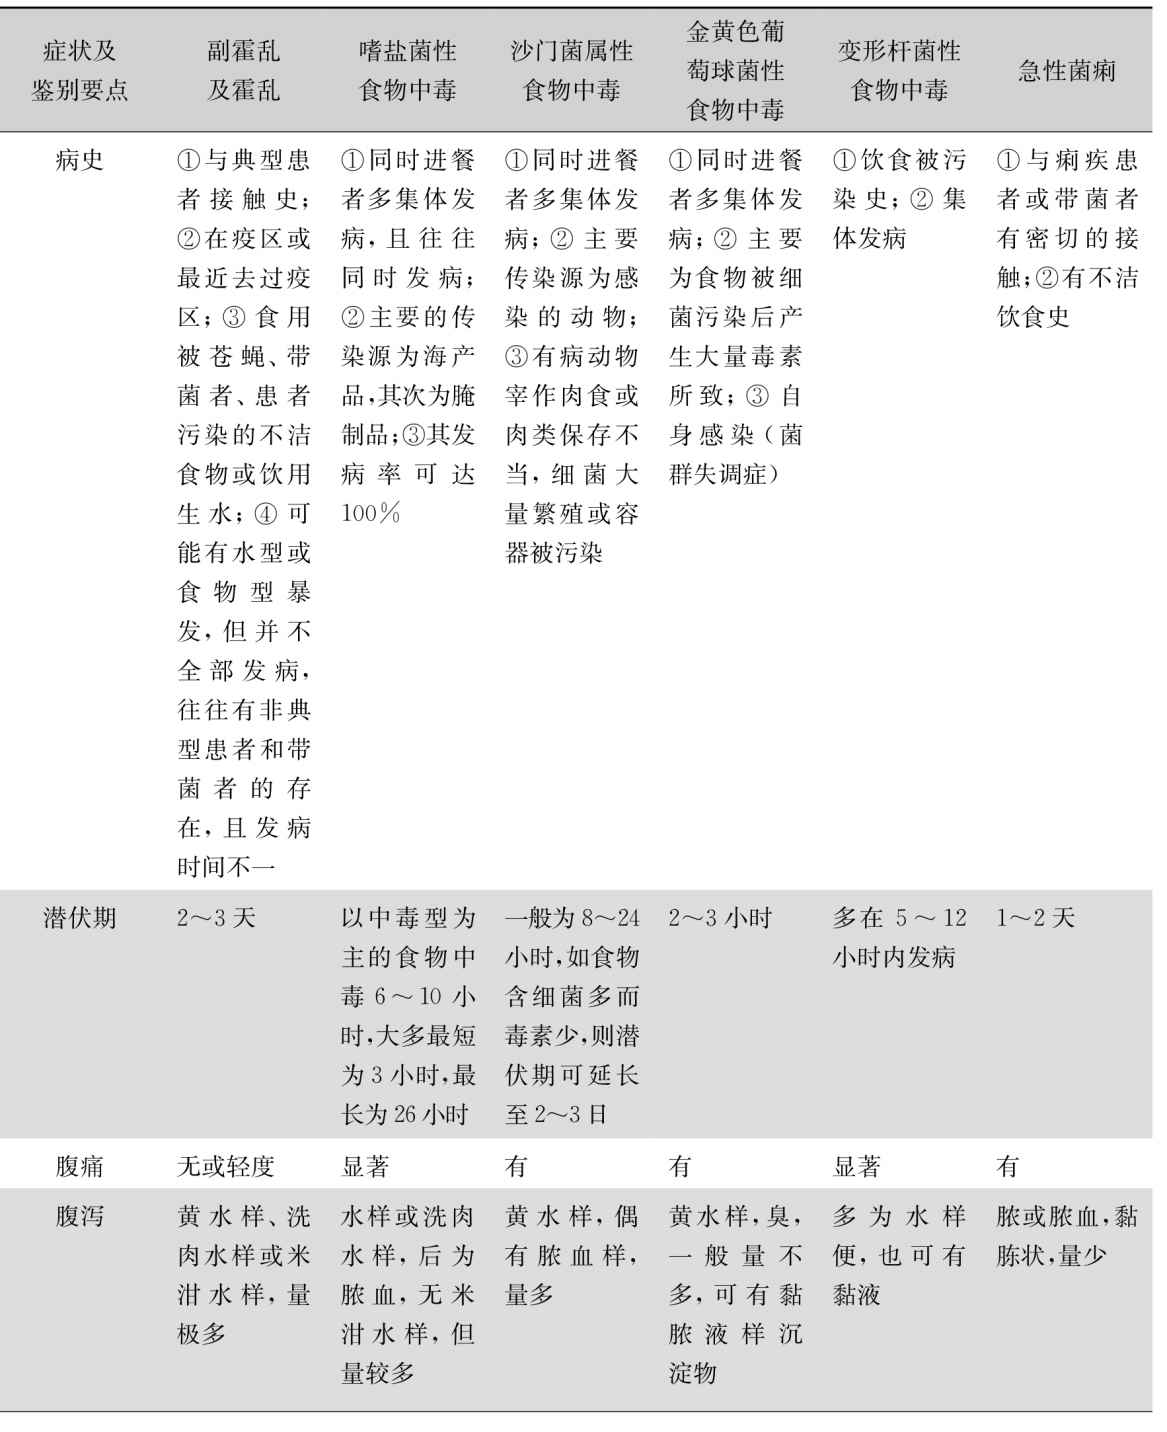
\includegraphics[width=\textwidth,height=\textheight,keepaspectratio]{./images/Image00128.jpg}\\
 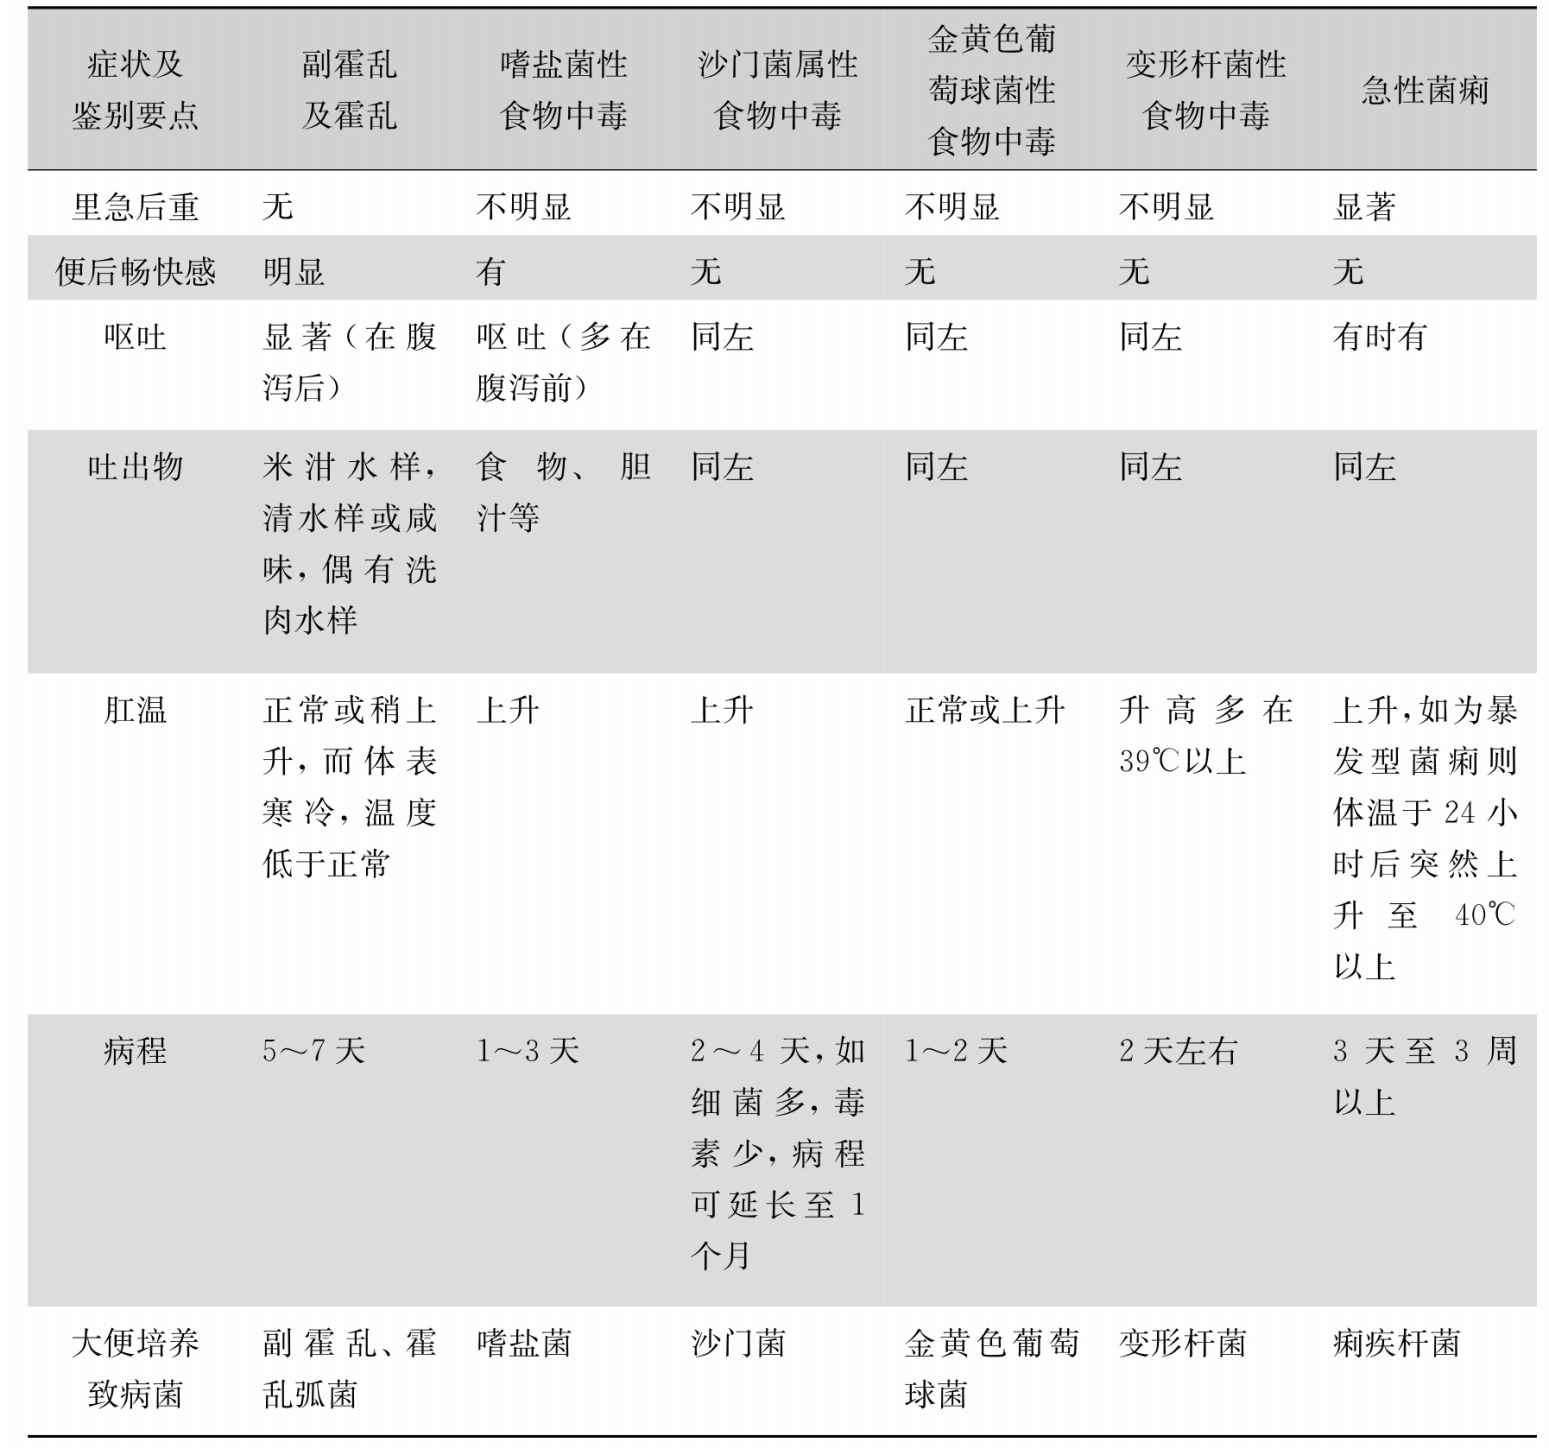
\includegraphics[width=\textwidth,height=\textheight,keepaspectratio]{./images/Image00129.jpg}
 \end{longtable}

\subsubsection{二、金黄色葡萄球菌性食物中毒}

产肠毒素性金黄色葡萄球菌,是较常见的细菌性食物中毒病原体之一。潜伏期甚短,一般于进食后2~3小时发病,病例暴发非常集中。患者均有不同程度的急性胃肠炎症状,恶心、呕吐最为突出而普遍,腹痛、腹泻次之。部分病例尚有发热、头晕、出汗、四肢麻木等症状。个别病例出现酸中毒与休克。病程一般为1~2天。预后良好。剧烈呕吐者可导致严重失水及继发性肾衰竭。

此病的临床特点是潜伏期短,病例暴发集中,来势凶猛,恢复迅速。由于金黄色葡萄球菌普遍存在于自然界中,正常人粪便中也可分离出此菌,因此单从患者粪便与食物中分离出此菌,不一定有诊断意义。另一方面,金黄色葡萄球菌肠毒素有相当的耐热性,即使食物在100℃中煮30分钟,仍不被破坏。虽然细菌已死亡,仍有可能中毒,此时标本培养虽为阴性,而未能排除金黄色葡萄球菌性食物中毒的可能性。因此,此病的诊断必须慎重,须结合流行病学调查、典型的临床表现以及细菌学检查结果,并排除其他原因所致的急性胃肠炎而确定之。

\subsubsection{三、变形杆菌性食物中毒}

变形杆菌可为食物中毒的条件性病原体,即在适于此菌繁殖和产生毒素的条件下有致病作用。潜伏期一般多为5~12小时,病程2天左右。国内报告流行最广的一组为2116例,此组的潜伏期中数为16.4小时,病程中数为15.2小时,预后均佳,无一例死亡。

变形杆菌性食物中毒的临床表现以急性胃肠炎为主,半数病例伴有发热、头痛。少部分患者除胃肠道症状外,可有过敏症状,如瘙痒、荨麻疹。诊断主要根据较短的潜伏期与病程,急性胃肠炎症状,并从食物与患者粪便中分离出菌型一致的变形杆菌,以及用获得的变形杆菌为抗原,做患者血清凝集反应,患者组较健康对照组凝集效价明显增高等特点。

此病与沙门菌属性食物中毒的主要临床区别点是:前者腹痛、腹泻较恶心、呕吐多见,病程大多不超过两天,预后佳良;后者病程多为2~4天,有死亡病例(早期由于败血症或休克致死)。

国内报告一组莫根变形杆菌性食物中毒病例潜伏期为19~45小时,平均为33小时。发病突然,有倦怠、乏力、恶心、腹泻与剧烈腹痛,但无里急后重,约35\%患者伴有呕吐。患者排黏液稀便,有时带血,气味腥臭。常有不同程度的发热,可达40℃或以上。少数重症患者有昏睡、脱水、酸中毒。病程3~4天。国内另一组病例报告,发病157人,发病率为74\%,病死率为8.3\%。诊断须根据:①上述的临床表现;②食物及粪便中检出莫根变形杆菌;③患者和未发病的同进食者血清与分离菌进行凝集反应,凝集效价明显增高,而健康对照组血清凝集反应阴性或低度阳性。

\subsubsection{四、嗜盐菌性食物中毒}

嗜盐菌引起的食物中毒在沿海一带颇为多见,病原体为一种嗜盐性细菌,学名为肠炎假单胞菌(Pseudomonasenteritis)。

此病主要流行于夏秋季,由于食用污染的海产品(章鱼、带鱼、墨鱼、蟹等)、肉禽类腌制品等所引起。潜伏期短,最短3小时,最长26小时,一般9~20小时。主要症状为腹痛、腹泻、发热、呕吐等。腹痛一般较其他急性肠道感染为重。腹泻每天三数次,10次以上少见,粪便呈血水样的情况较其他食物中毒为多见,也可呈水样或带脓血。粪便带血与黏液是常见的临床特征之一,半数以上病例被误诊为“痢疾”。文献报道重症患者有血压下降甚至休克。病原菌在粪便中消失特别快,多数在第二天即转为阴性,仅少数持续2~4天。病程一般为1~3天。诊断须根据流行病学调查,上述的临床表现以及疾病早期从粪便中分离出嗜盐菌,或(及)病期1~2天患者血清对嗜盐菌凝集效价增高(1∶80~320),一周后常显著降低或消失,最长者可持续两周。

菌痢型嗜盐菌性食物中毒易与细菌性痢疾混淆,下列几点有助于临床鉴别的参考:①前者可有集体发病史,可疑食品常为蟹、鱼等海产品;②前者腹痛较剧,一般多在脐周,少有里急后重,发热不如后者严重,但脱水现象较后者多见,而后者腹痛多在左下腹或中下腹,其程度虽有时较重,但少有以此为主诉而就医者。此病伴有血水样便时须与急性出血性坏死性肠炎或过敏性紫癜相区别。急性出血性坏死性肠炎为散发性,腹痛较为严重,中毒性休克较常见,左上腹或左中腹常有比较固定的压痛与肌紧张,肠鸣音常减弱。过敏性紫癜除血性便与腹痛之外,常有皮肤紫癜与血中嗜酸性粒细胞增多,也可有关节痛。个别嗜盐菌性食物中毒粪便呈黄水样者,须与沙门菌属或其他细菌所致的食物中毒、霍乱、败血症、中毒性肺炎等相区别。其他细菌性食物中毒并发休克者较少。霍乱患者的脱水现象较嗜盐菌食物中毒严重,腹泻次数也较多,大便量多,呈米泔水样,腹痛轻微或缺如,常无发热。败血症或中毒性肺炎伴休克者腹泻一般不严重,更少有剧烈的腹痛。

\subsubsection{五、肉毒杆菌性食物中毒}

本病由进食被肉毒杆菌毒素污染的食物引起,发病多由于进食罐头食品、发酵馒头、臭豆腐和豆瓣酱等被肉毒杆菌污染的食物所引起。此菌的外毒素对周围神经有特殊的亲和力。多数病例潜伏期为12~36小时,潜伏期愈短,则病情愈重,病死率愈高。其临床特点是:①前驱症状一般较轻,极少数有胃肠道症状,可能与食品种类有关。多数患者起病缓慢,有纳差、乏力、头晕、头痛等。少数有恶心、呕吐、腹胀、腹泻或便秘等胃肠道症状;②神经系统症状:患者体温、血压正常,神志清楚,感觉无障碍。典型症状及体征为对称性多数脑神经麻痹,可与前驱症状同时发生,多在其后出现眼部、口咽症状,面肌及呼吸肌等麻痹症状,它们并非单独出现,而是先后或交替出现。经抗毒治疗后其症状消失顺序与出现顺序恰好相反。本病的诊断依据是:①有进食可疑食物史;②出现进行性脑神经对称性麻痹;③可疑食品、血及大、小便均检出肉毒毒素,大便及可疑食品中能分离出肉毒杆菌;④用可疑食物滤液进行动物接种,实验动物的中毒表现和肉毒杆菌阳性。本病应与有机磷中毒、阿托品中毒、重症肌无力、多发性神经炎、低钙血症等鉴别。

\subsubsection{六、副溶血弧菌性食物中毒}

本病的病原菌为嗜盐杆菌或致病性嗜盐菌,海产品的带菌率很高,是夏秋季沿海地区食物中毒的重要致病菌,亦可通过各种污染的盐腌制品或咸菜、腌肉、咸蛋、酱菜等传播。潜伏期平均为6~12小时,短者不到1小时,长者可达100小时。起病急骤,初期有腹部不适,全身寒战,有阵发性加剧且部位不定的腹痛,伴恶心、呕吐,继之发热、腹泻,便次多少不一,多为每日7~8次,为水样便、糊状便、洗肉水样便或脓血便。白细胞总数轻度增加,中性粒细胞略升高。大便常规检查结果类似细菌性痢疾,大便及呕吐物在病初1~2天可培养出此菌。可疑食品中亦可分离出该弧菌。在流行季节进食可疑食物、集体发病、起病急骤、有腹痛腹泻发热等典型临床表现即可临床诊断。病原菌培养阳性可确定诊断。本病与细菌性痢疾的区别是:①前者有集体发病史,并进食过海产品;②前者腹痛较剧烈,一般多在脐周,少有里急后重,发热不如后者严重,但脱水现象较后者多见。后者腹痛多在左下腹或中、下腹,程度较轻。

\subsubsection{七、致病性大肠杆菌性食物中毒}

致病性大肠杆菌引起小儿与成人腹泻,国内有报告。此病可以食物中毒或医院内交叉感染的形式出现。国外文献也有报告,食物中含有一定量活的某些类型大肠杆菌,可引起成人的急性胃肠炎。在这些病例中,从食物与患者排泄物中均分离出致病性菌株,生物学和血清学检定均证明一致,用分离出的菌株做作患者血清凝集试验效价甚高。国内发病以5、6月最多,多因不洁饮食而致病,主要症状为腹泻,少数有发热、腹痛。目前认为,温带地方居民在热带地区罹患的“旅行家腹泻”,病原菌亦为致病性大肠杆菌。

\subsubsection{八、铜绿假单胞菌性食物中毒}

铜绿假单胞菌在自然界中分布甚广,食品受其污染机会很多,但食品污染后造成食物中毒事件的报道还不多见。铜绿假单胞菌性食物中毒在广东省曾有一组病例报告,患者以一岁以下婴儿最多,但成人也可罹患。小儿腹泻每天可达10次以上,并可引起脱水。大便多为水样、蛋花样。发热比一般腹泻者少见。有人认为小儿腹泻发病急、脱水快,用一般抗生素无疗效,须注意铜绿假单胞菌性食物中毒的可能性。食物及粪便中分离出铜绿假单胞菌可确定诊断。

\subsubsection{九、韦氏杆菌(耐热型)性食物中毒}

韦氏杆菌(B.Welchii,Cl.perfringens)食物中毒国外并不少见,但国内尚无报告。引起食物中毒者主要为A型和F型(中毒型),其中以A型最为多见。

潜伏期一般为8~20小时,短者仅3小时,长者可达50小时。主要通过受污染的食物传染,尤其是肉类与海产类食品。中毒多为集体发病,散发性甚少。主要临床表现是急性胃肠炎症状,腹痛、腹泻最为常见,腹泻每天数次至十几次,一般为稀便及水样便,很少为脓血便。其他症状为发热、呕吐、头痛、倦怠等。重病者可出现休克、痉挛、意识障碍以及肠出血坏死等现象。

韦氏杆菌菌型与临床表现有密切关系:由F型引起的食物中毒症状较为严重,呈出血性坏死性肠炎的临床表现,预后较差;由A型引起的中毒症状,则一般较轻,病程较短,预后良好。

韦氏杆菌性食物中毒的诊断主要根据流行病学调查,患者的临床表现以及可疑食物与患者呕吐物及粪便细菌学检查,确定病原菌的存在。

F型韦氏杆菌性食物中毒与急性出血性坏死性肠炎不易鉴别,也有人认为后者是由该菌引起的,但急性出血性坏死性肠炎为散发性,食物与大便中不一定能检出该菌。

\subsubsection{十、蜡样芽胞杆菌性食物中毒}

蜡样芽胞杆菌是一种需氧、有芽胞、革兰氏阳性杆菌,能产生不耐热的肠毒素和耐热的呕吐毒素。引起此种食物中毒的食品主要为含淀粉较多的谷类食物,如隔夜剩饭等。主要临床表现有突然起病,恶心、呕吐,腹痛、腹泻等。病情较轻,呈自限性,预后良好。

\subsubsection{十一、真菌性食物中毒}

真菌性食物中毒,主要是指由麦角菌、镰刀菌、青霉菌等所致的食物中毒。这些真菌是引起粮食作物发生病害的病原菌,粮食可在田间或保管不当而受污染,人畜进食受污染的谷物即可致病。

这类食物中毒与大多数的细菌性食物中毒不同,其毒性物质的产生是在真菌进入人体之前,且不被高温所破坏,因此在食品加热过程中,一般不能起消毒的作用。

真菌性食物中毒的潜伏期短,症状甚至可于半小时内出现,其临床表现因菌种不同而异,主要是胃肠道症状(呕吐、腹泻、上腹灼热感等)与中枢神经系统症状(头晕、头痛、烦躁、不安、惊厥、昏迷等)。由赤霉菌侵袭麦粒后导致的食物中毒,引起迷走神经刺激作用很明显,如头晕、恶心、流涎、腹痛、腹泻、冷汗、颜面潮红、步态蹒跚等症状,具有一定特征性。但也有引起造血系统、肝、肾、周围血管等病变和症状者,严重病例可因周围循环衰竭或呼吸麻痹而致死亡。

诊断主要根据胃肠表现及神经系统症状,从被污染食物中检出致病性真菌,必要时做动物毒性实验。

\protect\hypertarget{text00184.html}{}{}

\subsection{73.2 急性肠道感染}

\subsubsection{一、病毒性腹泻}

\paragraph{(一)轮状病毒性肠炎}

轮状病毒是最常见的腹泻病毒,是夏秋季婴儿腹泻的主要病原,主要经粪-口传播感染。该病毒分为七个组,其中只有A、B、C组能感染人。A组轮状病毒主要侵犯婴幼儿,起病较急,首发症状为发热、腹泻,部分患者为呕吐和咳嗽。轻至中度发热,1/3患儿伴有39℃左右的发热,大便每日十余次至数十次,水样便或黄绿色稀便,无黏液和脓血,有酸臭味。半数患者出现流涕、轻咳等上呼吸道感染症状,且先于腹泻出现,部分伴有支气管炎或肺炎。发热和呕吐2天后消失,腹泻可持续3~5天或1周,少数可达2周。40\%~80\%有轻、中度脱水,大多为等渗性,其次为高渗性,少数为低渗性。呕吐、腹泻严重者可出现重度脱水、酸中毒和电解质紊乱,甚至发生弥散性血管内凝血(DIC)及多器官衰竭。平均病程7天,可自愈。少数可迁延不愈,形成慢性腹泻,导致营养不良。重复感染普遍存在,同型及不同型别病毒均可重复感染。B组轮状病毒感染多为成人,称成人腹泻轮状病毒(ADRV)。感染后突然出现中等程度的腹泻,每日大便10次左右,重者每日超过20次,绝大多数为水样便,持续6~7天,呈自限性。病初2~3天伴有恶心、呕吐、腹痛、腹胀、乏力等,有轻度脱水。部分患者可有呼吸道症状,发热者很少。C组轮状病毒主要侵袭儿童,症状与A组感染相似,但持续时间较长。诊断主要根据临床表现及当地流行季节,婴幼儿应考虑A组;成人则应考虑B组;散发病例应考虑C组的可能。确诊主要依靠病原学检查,粪便浸液通过电镜见到特殊车轮状病毒颗粒即可确诊。也可做单克隆抗体检测,血清特异性IgA抗体滴度明显增高,也有诊断价值。

\paragraph{(二)肠腺病毒肠炎}

腺病毒主要引起呼吸道感染,但40型和41型主要侵袭小肠而引起肠炎,该病毒被WHO确认为引起儿童病毒性腹泻的第二重要病原。全年均可发病。肠腺病毒主要感染空肠和回肠,感染部位肠黏膜绒毛变短、变小,感染细胞核内出现包涵体,继之细胞变性、溶解,使小肠吸收功能障碍而引起渗透性腹泻。临床表现:潜伏期3~10天,平均7天。常先出现1~2天呕吐,继之水样腹泻,每日数次至数十次,持续1~2周,平均8~9天,少数可延续3~4周。近半数患者伴2~3天低热。20\%患者同时有鼻炎、咽炎、气管炎等上呼吸道症状。41型腺病毒引起的腹泻持续时间较长,而40型发病初期症状较重。周围血白细胞可轻度升高,大便镜检有白细胞。确诊有赖于病原学检查:①电镜或免疫电镜检测粪便中的病毒,但肠腺病毒在粪便中量少,阳性率不高,而且不能直接区分粪便中的其他种类腺病毒;②采用ELISA或间接免疫荧光法从粪便中可检测到病毒抗原;③核酸杂交或PCR从粪便中检测到病毒核酸,后者阳性率可达56\%,明显优于病毒分离。

\paragraph{(三)诺瓦克病毒肠炎}

全年均有发病,以冬季较多。从每年9月至次年4月,在密切接触的集体单位内突然暴发腹泻或呕吐,类似食物中毒,应考虑本病。成年人发病多见,该病大多数以腹泻或腹部痉挛性疼痛开始。大便每日4~8次,量中等,呈水样或稀粪便,无黏液及脓血。常伴有恶心、呕吐。少数病例仅有腹泻或仅有呕吐。12岁以上患者腹泻较多见。半数病例有中度发热或低热,可有全身不适、头痛、肌痛。病程持续1~2天,恢复后无后遗症。诊断依赖粪便中检出病毒抗原和血清抗体阳性。

\subsubsection{二、急性细菌性痢疾(急性菌痢)}

据近年国内成人感染性腹泻的分析,急性菌痢的致病菌以痢疾杆菌最常见,其他致病菌较少,依次为空肠弯曲菌、副溶血弧菌、沙门菌、白念珠菌、金黄色葡萄球菌等。

急性菌痢的病原菌目前以福氏与宋内痢疾杆菌为多见。发病多在夏秋季,往往形成大、小流行。潜伏期多为1~2天,长者可达7天。患者常以畏寒、发热和不适感急骤起病,体温可达39℃,可伴头痛、乏力、纳差,继而出现腹痛、腹泻,排便每天十余次至二、三十次,里急后重、恶心、呕吐与脱水。粪便初呈水样,以后排出脓血样或黏液血样便,里急后重更明显,大便量少,出现左下腹压痛和肠鸣音亢进,粪便镜检可见大量红、白细胞。取患者新鲜大便送培养检查,易检出痢疾杆菌。

中毒型菌痢以体质较好的儿童多见,成人甚少罹患。成人中毒型菌痢多发生于年龄较大、体质衰弱、营养欠佳的人。由于毒血症、呕吐和腹泻,休克出现较早而较重,中枢神经系统中毒症状并不少见。诊断须依据上述临床特点与粪便检查。

中毒型菌痢有时以高热、抽搐等毒血症症状为表现,可出现休克和(或)中毒性脑病,消化道症状可不明显。若患儿尚未排出脓血样便,以棉花竹签涂拭直肠,即有脓血黏着,镜检可见大量红、白细胞,培养发现痢疾杆菌,即可确定诊断。

急性细菌性痢疾与其他致病菌性肠炎的鉴别只能依靠粪便培养。

急性细菌性痢疾与急性阿米巴性痢疾的鉴别可参考表\ref{tab23-5}。

\begin{table}[htbp]
\centering
\caption{急性细菌性痢疾与急性阿米巴痢疾的鉴别}
\label{tab23-5}
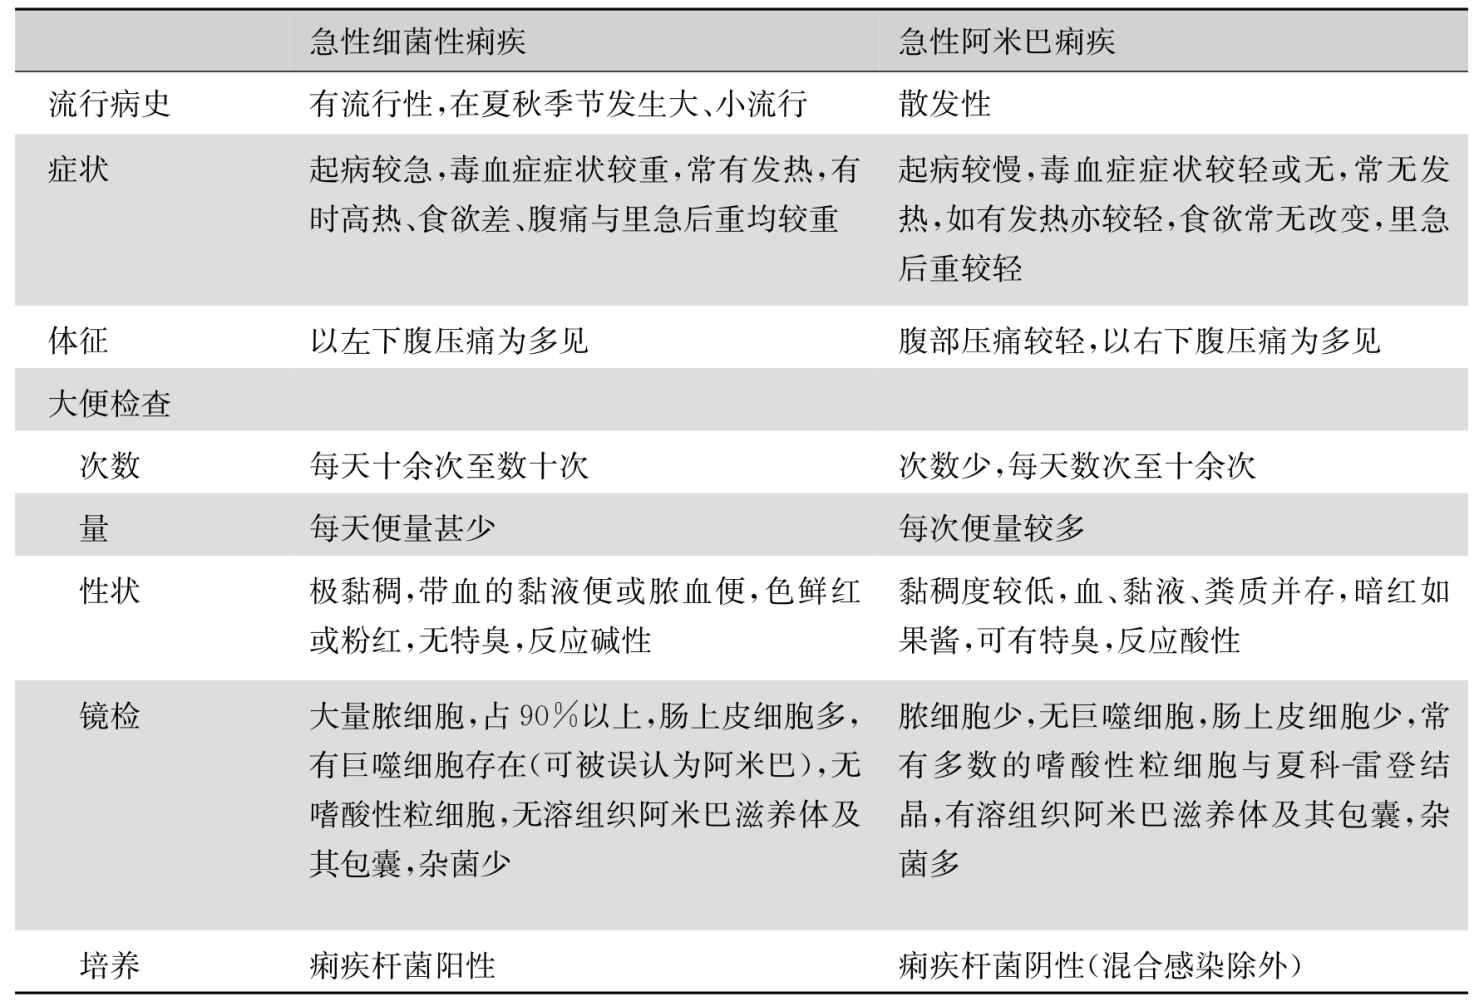
\includegraphics[width=5.9375in,height=4.03125in]{./images/Image00130.jpg}
\end{table}

\subsubsection{三、霍乱、副霍乱}

副霍乱系由ElTor弧菌所引起,其流行特点与真性霍乱(霍乱)不同,大多为地方性流行,并为散发性或跳跃式。此菌的培养特点、所引起的临床症状与病理改变均与霍乱弧菌所致者相同。霍乱在我国以夏秋季为流行季节,有分布在沿海沿江为主的地理特点。

霍乱的潜伏期一般为2~3天,也可短至数小时或长达6天之久。发病急骤,呕吐与腹泻均剧烈。初排出黄色稀便,继而成为典型的米泔水样,呈无粪质的灰白色浑浊液体。腹泻不伴有腹痛与里急后重,每次排便量甚多。呕吐常为喷射性,反复不止,呕吐物也呈米泔水样(吐泻期)。由于剧烈的腹泻与呕吐,患者呈严重的脱水状态,体温下降,四肢厥冷,皮肤起皱纹。常有肌肉痉挛,尤以腓肠肌与腹肌为明显。患者渐出现血压下降,脉搏微弱(休克期),重症者如不及时救治往往死亡。

如患者周围循环衰竭现象较轻,则渐趋康复。如周围循环衰竭现象持续较长、中毒严重,则常出现发热性反应(反应期)。患者可有持续高热,少尿或无尿,最后发展为尿毒症与酸中毒,可因急性肾衰竭而死亡。

霍乱主要须与副霍乱及各种原因的细菌性食物中毒相区别。霍乱与副霍乱的区别主要根据特殊的细菌学与血清学检查。轻型霍乱临床上与一般细菌性食物中毒难以区别,主要须根据大便培养检查。流行期间,粪便涂片染色、动力试验及制动试验可作为快速诊断方法。

确定诊断应符合以下三项之一:①有泻吐症状,粪培养有霍乱弧菌生长者。血清抗体阳性也有诊断意义。②流行区人群,有典型症状,但粪培养阴性,经血清抗体测定效价呈四倍或四倍以上增长。③虽无症状但粪培养阳性,且在粪检前后五日内曾有腹泻表现,并有密切接触史者。

\subsubsection{四、大肠杆菌性肠炎}

大肠杆菌是人类肠道内的正常菌群,是一种条件致病菌,与人类腹泻有关的主要有以下五类:产肠毒素性大肠杆菌(ETEC)、肠致病性大肠杆菌(EPEC)、肠侵袭性大肠杆菌(EIEC)、肠出血性大肠杆菌(EHEC)、肠黏附性大肠杆菌(EAEC)。其中ETEC、EPEC及EAEC对小肠上段具有亲向性,引起小肠分泌而对肠组织无侵袭的倾向,临床上主要产生水样便,无脓血;而EIEC与EHEC大多侵犯结肠,引起侵袭性病变,开始为水样便,继之产生脓血便或血性便。诊断:主要为临床诊断,肠致病性大肠杆菌(EPEC)性肠炎主要发生在婴儿。ETEC是部分旅游者腹泻的病原体。EAEC则与世界各地慢性腹泻有关。

\subsubsection{五、耶尔森菌性肠炎}

本病系由小肠、结肠炎耶尔森菌(Yersiniaenterocolitica,简称耶氏菌)引起的急性传染病。临床上以小肠炎最为常见,但临床症状因年龄不同而异,成人常有肠外表现,婴幼儿以肠道症状为主。潜伏期4~10天,无明显前驱症状,婴幼儿的主要症状为腹痛、腹泻、发热等急性肠炎的表现。>5岁的儿童和青少年可出现阑尾炎样症状。除上述症状外,亦有恶心、呕吐、纳差、无力、头痛、体重减轻等。免疫功能抑制或原有其他疾病者,可发生败血症,预后较差,病死率达50\%,临床表现为急性中毒、亚急性感染。败血症并发其他脏器的炎症,病程中可出现结节性红斑、关节炎、关节痛,偶尔并发眼部炎症、赖特综合征或心肌炎。本病完全不同于炎症性肠病和其他原因的肠炎。耶尔森菌分布很广,可自牛奶、奶制品、蛋制品、肉类及水产品中分离出来,家畜家禽排泄物中常带有此菌。凡进食疑有被污染的食物,或与感染的动物接触后出现腹泻、腹痛、发热、结节性红斑、关节炎,或有局灶脓肿形成的患者,应疑有本病可能。诊断主要依据从肠内容物中分离出本菌或血清抗体滴度测定。确定本菌感染最可靠方法的是细菌培养,检查程序一般是通过增菌分离培养,挑选可疑菌落进行鉴定。

\subsubsection{六、空肠弯曲菌肠炎}

本病系由弯曲菌引起的肠道传染病。潜伏期1~7天,平均4天。起病急,仅极少数患者有前驱症状(如全身不适,头痛、肌肉痛等)。其主要症状有发热,体温38~40℃、腹痛、腹泻、呕吐等,程度不一。腹泻初为水样便、黏液便,2~4天后多为血性或脓血便。腹痛剧烈,常呈上腹部或脐周阵发性绞痛。胎儿弯曲菌亚种感染者常有肠外感染症状,如脑膜炎、胆囊炎、心包炎、败血症等。个别病例,特别是免疫缺陷患者常表现出反复菌血症和慢性肠炎的经过。另外,本病常并发反应性关节炎、溶血性尿毒症综合征和赖特综合征。当地流行情况,如有无家禽、家畜接触史,是否摄入可疑污染的食物,血液厌氧菌培养可分离出本菌。急性期和恢复期血清凝集素效价>4倍亦有诊断价值。病程一般7~10日,也有长至6周者,少数可形成慢性腹泻。红霉素和氨基糖苷类抗生素治疗有效。

\subsubsection{七、抗生素相关性腹泻(假膜性肠炎)}

抗生素相关性腹泻是指应用抗生素后继发腹泻,为较常见的药物不良反应,其发生率视不同抗生素而异,约为5\%~39\%。按病情严重程度不同,分为单纯腹泻、结肠炎或假膜性肠炎。假膜性肠炎指病情严重,在结肠黏膜有假膜形成的特殊类型,如不及时给予合理治疗,可导致并发症,死亡率高达15\%~24\%。抗生素可抑制肠道的正常菌群生长,使一些条件致病菌(主要是难辨梭菌)得以快速繁殖,从而产生抗生素相关性肠炎,引起此类腹泻的抗生素以广谱抗生素[氨苄西林、羧苄西林、氨基糖苷类、林可霉素、头孢曲松钠(菌必治)、头孢哌酮钠(先锋必)、亚胺培南-西拉司丁钠(泰能)等]最常见,临床以水样或糊状便为主,多发生在应用抗生素治疗后10天内,大便每日4次以上,重者20~30次,大便中有时可见片状的黄白色膜状物,伴有发热、腹痛、腹胀、毒血症,若不及时诊治,可出现中毒性巨结肠、肠梗阻、肠穿孔等并发症。诊断:病人在应用抗生素过程中,如出现腹泻,应警惕本病的可能。单纯腹泻病人症状轻微,结肠无假膜形成,停用有关抗生素后,腹泻自行好转。假膜性肠炎病人症状较重,每日有5次或5次以上的不成形便,可无肉眼血便或黏液便,这些病人大多有难辨梭菌感染,腹泻同时伴有腹胀、腹痛,并有发热,有时被误认为原有感染性疾病的恶化,须注意。在病变的发展中,可出现难以忍受的腹痛,类似急腹症。如持续用有关抗生素,则症状加重,可伴脱水、电解质紊乱,大量清蛋白丢失,甚则死亡。大便厌氧培养出难辨梭菌可确诊。95\%假膜性肠炎患者难辨梭状杆菌毒素检测阳性。结肠镜检查:病变为肠壁弥漫性炎症,覆有大小不一的黄白色斑块状假膜,通常为2~10mm宽,也可融合成片。病变常位于左半结肠,乙状结肠和直肠较多见,假膜脱落后似溃疡样改变。

\subsubsection{八、白念珠菌性肠炎}

白念珠菌属机会性致病菌,普遍存在于人体的体表开口处,如口腔、鼻腔、咽部、上呼吸道、消化道、肛门、外阴和皮肤上。当机体免疫力低下时,寄生于肠道的白念珠菌侵袭肠黏膜,引起肠炎。以营养不良、身体衰弱幼儿多见。患者的大便呈稀糊状或水样,夹带黏液,严重者呈黏液血便或脓血便,大便次数每日3~15次不等,多伴有腹痛,腹泻迁延不愈为本病的特点,可持续数月。长期大量应用抗生素或类固醇激素、免疫抑制剂治疗者出现大量水样腹泻,排除其他原因,应高度怀疑此病。粪便涂片发现大量念珠菌菌丝,尤其发现M型或伪菌丝念珠菌,结合临床即可诊断。念珠菌培养阳性率低,且阳性意义常难肯定。肠镜检查可见肠黏膜糜烂,有小的溃疡,在溃疡面上有白色假膜覆盖,活检标本可发现念珠菌的Y型和M型。血清抗体,抗原检测对诊断有一定意义,但须与临床相结合。因其临床表现为非特异性,常与其他致病性或条件致病性真菌或细菌混合感染,有时诊断十分困难。因此,必须根据流行病史、临床表现、粪便真菌学及肠镜检查结果综合分析,方可作出诊断。抗真菌药物治疗有效,也能进一步证实诊断。

\protect\hypertarget{text00185.html}{}{}

\subsection{73.3 急性肠寄生虫病}

\subsubsection{一、急性阿米巴肠病}

阿米巴病是人类感染溶组织阿米巴原虫引起的疾病,其中以肠阿米巴病为主,表现为肠炎或痢疾,并可引起肠外并发症。本病流行于世界各地,以热带和亚热带地区为多见,感染者中约有5\%~50\%为无症状带虫者,潜伏期为1~8周,一般为5~9日。临床表现多种多样,其表现取决于感染部位、感染的数量、肠道菌群状态、人体健康状况等。一般起病较慢,以腹痛、腹泻为主要症状,大便每天数次至十几次,甚少超过20次。全身中毒症状较轻,右下腹常有轻压痛,常无发热。因阿米巴肠病临床症状与其他腹泻病无明显区别,且各临床型的表现差异很大,故仅凭临床表现很难作出确切诊断,因此,对原因不明的腹泻,经抗生素治疗无效者,应进一步反复进行病原学检查以明确诊断。

实验室诊断:①粪便检查:典型粪便呈暗红色果酱状,有粪质、带脓血和黏液,有腥臭。显微镜检查可见成串聚集的陈旧红细胞、脓细胞。新鲜粪便脓血中易找到大量阿米巴滋养体,粪质部分涂片碘染色可找到包囊,常见有夏科-雷登晶体。采用PCR技术检测粪便中溶组织阿米巴原虫的DNA,是一种特异性强、敏感性高的诊断方法。②血清学检查:临床高度怀疑,但粪便原虫检查阴性者可采用免疫荧光、酶联免疫吸附法、间接血凝法等进行血清学检查,对肠内和肠外阿米巴病,血清学检测阳性率可达90\%。③乙状结肠镜检查:肠镜下可见溃疡表浅,大小不一,溃疡与溃疡间的肠黏膜多正常,典型的溃疡为散在的长圆形或圆形,边缘隆起充血。溃疡表面分泌物涂片可查到滋养体。④X线检查:钡灌肠X线检查对肠道狭窄、阿米巴肉芽肿等有一定的诊断意义。⑤治疗性诊断:对临床高度怀疑者,经上述检查仍不能确诊者,可给予抗阿米巴药物治疗,如疗效显著有助于诊断。

暴发型阿米巴肠病病情凶险,患者有严重中毒症状和严重腹泻,粪便呈米汤样乃至血水样,常混有片状黏膜脱落,恶臭。伴明显腹绞痛、里急后重甚至脱肛。粪便镜检可发现阿米巴滋养体。

\subsubsection{二、隐孢子虫病}

隐孢子虫(CSO)病是由微小隐孢子虫引起的人畜共患肠道传染病。腹泻是其主要症状,表现为水样便,或带泡沫和少量黏液。根据机体免疫功能不同,病情轻重有很大差别,免疫功能正常者,短期内自愈;免疫功能低下者,腹泻重且持续时间长,甚至死亡。

实验室检查:从大便或肠黏膜活检标本中查卵囊:①涂片染色:留取大便,经沉淀法或直接涂片用金胺酚-改良抗酸复染法染色,光学显微镜检查,阳性率较高,简易可行。②间接免疫荧光(IFAT)法:以单克隆抗体,用IFAT法,检测粪便中卵囊,敏感性比染色法高10倍,快速,20~30秒可出结果。③PCR法查卵囊:其检查阈值为每克粪便中含500个卵囊,敏感性比染色法提高100倍。④PCR结合地高辛标记的寡核苷酸探针法,敏感性比染色法提高5000倍,检测阈值相当一个卵囊的DNA含量,为目前敏感性、特异性均最强的方法。

血清抗体检测:采用ELISA或IFAT法,检测CSO特异性抗体IgG、IgA、IgM病后2~5周开始出现,持续约1年,与其他球虫目寄生虫无交叉免疫。免疫功能正常者,恢复期抗体滴度高,AIDS患者血中也有低水平循环抗体,但低丙种球蛋白血症者,抗体阴性。

诊断:凡原因不明之水样泻患者,来自农村,年龄在5岁以下,或因AIDS等致免疫功能低下者,均应疑及本病。从粪便或肠黏膜上发现CSO即可确诊。

\subsubsection{三、急性血吸虫病}

日本血吸虫病是日本血吸虫感染后寄生在人体门静脉系统引起的寄生虫病。在我国广泛流行于长江以南及沿岸地区。人感染后表现复杂多样,根据感染的轻重、病期早晚、虫卵附着部位以及机体免疫反应不同,可分为急性和慢性两种。临床表现急性期有发热、体温多在38~40℃,呈间歇热或弛张热型,伴畏寒、盗汗、腹痛、腹泻,大便次数不多,为稀水样便,继之为脓血便,类似痢疾样大便,有里急后重及局限性压痛。肝、脾大,有压痛,常伴有变态反应症状,如荨麻疹、血管神经性水肿、咳嗽、哮喘等症状。慢性血吸虫病常伴有贫血和肝、脾大。主要依据患者粪便中检出虫卵或结肠镜检查作黏膜活检发现虫卵明确诊断。

\protect\hypertarget{text00186.html}{}{}

\section{74 急性中毒}

\subsection{74.1 植物类急性中毒}

\subsubsection{一、“臭米面”中毒}

“臭米面”是东北地区农村将玉米等粮食,用水浸泡发酵制成,可制成各种食品,有时进食后可引起中毒。病因与发病机制尚未明确,初步认为是某些真菌和细菌的混合毒素所致。一般在食后数小时至十几小时发病,出现胃部不适、恶心、呕吐、腹胀、腹痛等症状,腹泻与食欲不振也常见。严重者可发生黄疸、神经精神症状(嗜睡、狂躁或昏迷)、心脏损害、休克及急性肾衰竭,表现为多个器官损害的症状。此病一旦发生,病死率甚高。

\subsubsection{二、发芽马铃薯中毒}

马铃薯在萌芽时期,幼芽含有大量龙葵碱,在皮质内含量尤多,龙葵碱对黏膜有腐蚀性,破坏细胞,重者致脑水肿或呼吸肌麻痹。食之可致中毒,出现头晕、头痛、喉干、发热、恶心、呕吐、腹痛、腹泻等症状。轻者1~2日可自愈,严重者发生呼吸困难、惊厥与昏迷,可因呼吸中枢麻痹而死亡。

\subsubsection{三、白果中毒}

白果毒性以绿色的胚为最剧,共肉质外种皮含有的毒性成分为银杏酚、白果酚、白果酸、氢化白果酸、氢化白果亚酸等,种仁含有微量的氰苷。大量进食后可引起中毒。中毒多发生于儿童,潜伏期1~12小时不等。中毒的主要表现是呕吐、腹泻、烦躁不安、发热、呼吸困难、发绀、惊厥;昏迷、瞳孔对光反应减弱或消失等。少数病例可出现末梢神经功能障碍的症状。脑脊液检查可有细胞增多与蛋白阳性反应。

\subsubsection{四、火麻仁中毒}

火麻仁(大麻仁)是润下药,剂量每服为9~15g。有人曾服用大量(60~120g)而引起中毒症状。食入量愈多则症状愈重,表现为恶心、呕吐、腹泻、四肢麻木、定向力消失等症状。重症病例出现瞳孔散大、抽搐与昏迷。

\subsubsection{五、毒蕈中毒}

毒蕈种类甚多,有些外观上与无毒者相似,误食之而致中毒者也有报告。中毒多发生于夏秋季。症状最早可于食蕈后数分钟出现。最迟的达18小时。其主要表现是急性胃肠炎、中毒性肝炎、溶血、精神异常与中枢神经损害的症状。早期出现大汗、流涎、流泪、瞳孔缩小等迷走神经兴奋症状。胃肠症状表现为恶心、呕吐、腹痛与腹泻。重症病例发生呕血、便血、黄疸、紫癜、谵妄、抽搐与昏迷,预后多不良。

\subsubsection{六、菜豆中毒}

菜豆又称扁豆、四季豆、刀豆、豆角、芸豆,中毒大多由于进食大量储存过久、烧煮不透的菜豆所致,多发生于秋季。毒性成分为皂素。发病急骤,可在进食后数分钟发病,潜伏期一般为1~5小时。主要表现为恶心、呕吐、腹痛、腹泻,也可出现头晕、头痛、四肢麻木等症状;部分患者有胃烧灼感、胸闷、心慌、畏寒等,体温多正常或伴有低热。病程较短,一般为数小时到1~2天,预后良好。少数重症者可发生呕血或溶血性贫血。

\subsection{74.2 动物类急性中毒}

\subsubsection{一、河豚中毒}

河豚毒素具有箭毒样作用,可阻断神经肌肉冲动的传导,对胃肠黏膜有刺激作用。可作用于周围神经与脑干中枢,使之发生麻痹。首先引起周围的知觉神经麻痹,继而引起运动神经麻痹,最后才累及脑干中枢,如呼吸中枢麻痹可引起呼吸停止,血管舒缩中枢麻痹引起血压下降与休克。

河豚毒素主要存在于河豚的睾丸、卵巢、卵子、肝、血液,肌肉中无毒。潜伏期约l/2~3小时。主要表现为不适感、颜面潮红、上脸下垂、瞳孔缩小(后散大)、恶心、呕吐、腹泻、乏力等症状,口唇、舌尖、指端等处麻木。重症者出现轻瘫或瘫痪、语言困难、发音不正、脉搏细数。特别严重者可因呼吸麻痹或心搏停止而死亡。死亡率可高达50\%,重症病例心电图多呈不同程度的房室传导阻滞。诊断上主要根据有摄入河豚或与河豚混放在其他鱼中的病史,食后迅速发病,进展快,首先出现胃肠症状,很快出现神经麻痹和呼吸循环中枢麻痹。

\subsubsection{二、动物肝中毒}

进食大量的狗、狼、狍、鳇鱼、鲨鱼的肝引起急性中毒,国内曾有报告。其主要原因是动物肝含有大量维生素A。症状轻重与进食量成正比。多在进食后3~6小时起病,主要症状是乏力、头痛、厌食、恶心、呕吐,常伴腹痛、腹泻,并有皮肤潮红灼热与皮肤脱屑现象。血常规与肝功能试验正常。

\subsubsection{三、鱼胆中毒}

鱼胆中毒近年有多例报告,主要见于东南沿海地区,一般先出现胃肠道反应症状,继而(第2~3天)出现肝肾损害症状。胃肠道反应主要有:①腹痛,多位于上腹部或脐周;②呕吐;③腹泻,多为黄色水样便或稀烂便,无脓血,最多者每天10余次。继而出现中毒性肝实质细胞损害与不同程度的急性肾衰竭。本病在早期,须注意与细菌性食物中毒和其他原因的急性胃肠炎相鉴别。后期出现肝大、黄疸与少尿时,须注意与急性病毒性肝炎和其他原因的肝肾综合征相鉴别。一旦出现重症急性肾衰竭,应迅速作腹膜透析或人工肾透析。

\subsection{74.3 化学毒剂急性中毒}

\subsubsection{一、急性有机磷农药中毒}

急性有机磷农药中毒一般在有机磷侵入人体后12小时以内发病,大量口服时能在20分钟左右发病。发病初期先出现乏力、头痛、眩晕等非特异症状,以后渐次出现多汗、流涎、恶心、呕吐、腹泻、缩瞳、视力模糊等毒蕈碱样中毒症状。瞳孔缩小至针头大,呼气及排泄物有大蒜臭味。血清胆碱酯酶活性测定有助于诊断。

\subsubsection{二、急性锌中毒}

在镀锌的容器中存放酸性食物或饮料,锌即可以有机酸盐的状态,大量污染食物或饮料,人进食后即可引起中毒。国内报告曾有用镀锌铜壶或铁筒装酸性饮料引起急性锌(及铜)中毒的病例。其主要临床表现是恶心、呕吐、腹痛、腹泻等,但无发热。食物或饮料中锌含量测定可确定诊断。

\subsubsection{三、急性砷中毒}

急性砷中毒主要表现为恶心、呕吐、腹痛、腹泻、排黄色或灰白色水样便等急性胃肠炎症状。国内报告有用三氧化二砷塞药治疗阴道滴虫病,引起中毒致出现呕吐腹泻,被误诊为细菌性食物中毒,甚至引起死亡的病例。

\subsection{74.4 药物刺激及毒性反应}

灭虫宁、哌嗪、利血平、氟尿嘧啶、新斯的明、垂体后叶素、秋水仙碱、胍乙啶等均可引起腹泻,停药后迅速缓解。

\protect\hypertarget{text00187.html}{}{}

\section{75 全身性疾病}

\subsection{一、急性全身性感染}

败血症、流行性感冒、脊髓灰质炎、急性病毒性肝炎、麻疹、大叶性肺炎、钩端螺旋体病、回归热、伤寒与副伤寒等急性全身性感染,在病程(尤其是早期)中可发生轻度乃至中度腹泻,排糊样或水样稀便但无脓、血或黏液等成分,也不伴有腹痛。如胃肠症状较重,而其他系统病征尚未明显,早期可被误诊为细菌性食物中毒。

胃肠型疟疾罕见,主要症状是频繁而严重的恶心、呕吐、上腹痛,并有频繁的腹泻,排水样便。但也有报告偶尔呈痢疾样便,伴里急后重,血涂片未发现疟原虫前有被误诊为痢疾者。

\subsection{二、过敏性紫癜}

过敏性紫癜(出血性毛细血管中毒症)引起急性腹泻者并非少见。皮肤紫癜、血中嗜酸性粒细胞增多、大便反复涂片检查与培养阴性均有助于此病的诊断。少数病例早期或偶尔在全病程中不出现皮肤紫癜,仅表现急性肠炎症状,则可致误诊。血中嗜酸性粒细胞增多、止血带(束臂)试验阳性、多发性对称性关节肿痛等,均提示此病的诊断。内镜检查黏膜水肿,有散在或密集的黏膜瘀斑、糜烂及浅溃疡,以十二指肠、回肠末端及升结肠病变明显,严重者有肠腔内积血。

\subsection{三、变态反应性胃肠病}

变态反应性胃肠病(gastroenteropathia
allergica)系指某些健康者进食一般人能耐受的食物之后,引起急性胃肠症状,表现为呕吐、腹痛与腹泻,常伴有荨麻疹、偏头痛样头痛、血管神经性水肿等表现。引起变态反应性胃肠病的食物甚多,常见者为虾、蟹、海鱼、乳类、蛋类等,发病与个体过敏体质有密切关系。有些病例表现为急性嗜酸性粒细胞性胃肠炎。

菠萝过敏症也属于变态反应性胃肠病范畴,任何年龄均可罹患,而以儿童为多见,症状轻重与进食量多少未见明显的关系。食用不久(10分钟至2小时)即发生肠绞痛、恶心、呕吐、腹泻等急性胃肠炎症状,多伴有结膜充血、荨麻疹,重症者有不同程度的过敏性休克。

\subsection{四、移植物抗宿主病}

移植物抗宿主病是异基因骨髓移植的主要并发症。虽已采用一定的预防措施,但由于主要组织相容性复合物的多态性,仍有50\%~70\%患者移植后发生不同程度的移植物抗宿主病。急性移植物抗宿主病临床表现为广泛性皮疹、血清胆红素增高以及不同程度的腹泻,也有重症腹泻,伴肠绞痛。

\subsection{五、尿 毒 症}

纳差、恶心、呕吐常为本病之首发症状,且常随病情进展而加剧,呈顽固性,由此造成水、电解质代谢紊乱和酸碱失衡加剧,反过来又加重尿毒症的症状。60\%~70\%病例有胃、十二指肠症状,亦有肠黏膜出血、溃疡和穿孔发生。腹泻因尿毒症性结肠炎所致,呈水样大便,每日数次,一般不伴有腹痛。腹泻由于尿素分泌增加,细菌分解成氨刺激黏膜引起,也与胃肠道内多肽类激素水平增高和代谢障碍引起黏膜屏障功能降低有关。酸中毒、低血钠及中枢神经系统受损亦可引起或加重原有胃肠道症状。

\subsection{六、甲状腺危象}

系甲状腺功能亢进时出现的严重表现,可危及生命,早期时患者原有症状加重,伴中等发热,体重锐减,恶心、呕吐,以后发热可达40℃或更高,心动过速、大汗、腹痛、腹泻、甚至谵妄、昏迷。

\subsection{七、其 他}

\subsubsection{(一)急性出血性坏死性肠炎}

急性出血性坏死性小肠炎是由厌氧的产气荚膜梭菌(产生B毒素的Welchii杆菌)感染引起的急性肠炎。春秋季多见,儿童和青少年发病率较高。本病为急性起病,剧烈腹痛、腹胀,可伴有呕吐、腹泻,便量较大,多呈血水样便,血便持续2~6天,长者可达1个月左右。严重者有发热、感染中毒症状重,可出现休克、呼吸困难、少尿或无尿,急性肾衰及弥散性血管内凝血(DIC)等,合并有肠穿孔、腹膜炎者病情更凶险,病死率可达40\%~50\%。体检可见腹胀,脐周压痛,伴肠穿孔、腹膜炎者则有全腹压痛、肌紧张和反跳痛,甚至出现中毒性肠麻痹体征。

实验室检查:可有末梢血白细胞计数增高、核左移;粪便检查肉眼可见为血水样,镜下有红细胞和白细胞;污染食物及患者粪便细菌培养可获阳性结果;亦可有低血钾、代谢性酸中毒的实验室检查所见。其他如腹部X线检查可见有肠管扩张,有腹水者会出现肠管浮游等。急性期不宜作胃肠钡餐或钡灌肠检查,以免引起肠穿孔。

诊断:有不洁饮食史,临床上急性起病、发热、腹痛、频繁腹泻,血水样便者或腹痛后休克或麻痹性肠梗阻等应考虑本病,从粪便和(或)污染食物的培养中获产气荚膜梭菌则可确诊。

\subsubsection{(二)急性放射性肠炎}

以急性肠黏膜改变为特征,轻症者肠上皮细胞分裂象减少,柱状细胞进行性变平,一周后可见绒毛变短变钝,停辐射后两周内恢复正常。急性期主要表现为腹泻、排鲜红色血样便或黏液、里急后重及恶心、呕吐。累及小肠时有剧烈腹痛。严重者可发生溃疡而致严重便血或形成肠瘘,甚至穿通输尿管、子宫或其他肠管,损伤严重的肠黏膜再生不全,肠壁纤维组织增生变厚、短缩,以及肠袢间粘连而致肠狭窄,可有肠梗阻征象。极少数病例可发生放射性全结肠炎,表现为结肠、直肠广泛的浅而不规则溃疡,常有血性腹泻、蛋白质丢失、消瘦、贫血等与溃疡性结肠炎类似的临床表现。

诊断:急性放射性肠炎放疗期间(1~2周)如发生腹泻或伴有便血,首先考虑为放射性肠炎;可做结肠镜检查,如见受辐射肠段黏膜出血水肿、增厚及散见红斑,表面粗糙呈细颗粒状质脆接触易出血;重症如见糜烂、浅溃疡及渗血,溃疡周边有特征性毛细血管扩张改变,基本可以确诊。检查时应注意肠穿孔的出现。

\subsubsection{(三)急性溃疡性结肠炎}

溃疡性结肠炎(ulcerative
colitis,UC)的病变以结肠黏膜广泛连续性的溃疡糜烂为主,多累及远端结肠和直肠。临床表现为黏液脓血便或黏液血便、腹泻、腹痛、里急后重。病程多缓慢,反复发作。亦有急性暴发者,常为重症。急性发作时频繁腹泻、血便或水样血性便,每日可达10~30次,腹部持续性钝痛或剧痛,可有腹膜刺激征。可有发热、毒血症、脉速、消瘦、贫血、水电解质失衡和营养障碍。可并发中毒性巨结肠、肠大出血、肠穿孔等。实验室检查可有明显贫血、中性粒细胞增高、血沉加快、血清蛋白降低、低血钾等。粪便见脓、血、黏液,无虫卵、致病菌及真菌。内镜检查肠黏膜水肿充血、脆易出血,多发性糜烂及溃疡,表面覆盖血性渗出物或黄白色脓性物。急性期重症者暂缓内镜检查,以防穿孔。

结肠镜检查并活检是UC诊断的主要依据。结肠镜下UC病变多从直肠开始,呈连续性、弥漫性分布,表现为:①黏膜血管纹理模糊、紊乱或消失、充血、水肿、质脆、自发性或接触性出血和脓性分泌物附着,亦常见黏膜粗糙、呈细颗粒状;②病变明显处可见弥漫性、多发性糜烂或溃疡;③可见结肠袋变浅、变钝或消失以及假息肉、黏膜桥等。

病理表现:

活动期:①固有层内弥漫性、急性、慢性炎性细胞浸润,包括中性粒细胞、淋巴细胞、浆细胞、嗜酸性粒细胞等,尤其是上皮细胞间有中性粒细胞浸润和隐窝炎,乃至形成隐窝脓肿;②隐窝结构改变:隐窝大小、形态不规则,排列紊乱,杯状细胞减少等;③可见黏膜表面糜烂、浅溃疡形成和肉芽组织增生。

缓解期:①黏膜糜烂或溃疡愈合;②固有层内中性粒细胞浸润减少或消失,慢性炎性细胞浸润减少;③隐窝结构改变:隐窝结构改变可加重,如隐窝减少、萎缩,可见帕内特细胞(Paneth
cell)化生(结肠脾曲以远)。

无条件行结肠镜检查的单位可行钡剂灌肠检查。检查所见的主要改变为:①黏膜粗乱和(或)颗粒样改变;②肠管边缘呈锯齿状或毛刺样改变,肠壁有多发性小充盈缺损;③肠管短缩,袋囊消失呈铅管样。

在排除其他疾病基础上,可按下列要点诊断:①具有上述典型临床表现者为临床疑诊,安排进一步检查;②同时具备上述结肠镜和(或)放射影像学特征者,可临床拟诊;③如再具备上述黏膜活检和(或)手术切除标本组织病理学特征者,可以确诊;④初发病例如临床表现、结肠镜以及活检组织学改变不典型者,暂不确诊UC,应予随访。

\subsubsection{(四)伤寒和副伤寒}

伤寒是由伤寒杆菌引起的急性消化道传染病。主要病理变化为全身单核-巨噬细胞系统的增生性反应、回肠远端微小脓肿及小溃疡形成。典型病例以持续发热、相对缓脉、神情淡漠、脾大、玫瑰疹和血白细胞减少等为特征,主要并发症为肠出血和肠穿孔。

本病的病原为伤寒杆菌,属沙门菌属D组。典型伤寒潜伏期10天左右,自然病程约4周,可分为4期:①初期:相当于病程第1周,主要症状为发热,可有咳嗽、乏力、全身不适等症状。②极期:相当于病程第2~3周,常有伤寒的典型表现。高热持续不退,多数呈稽留热,持续约10~14日。部分患者有腹泻、便血,部分患者可有便秘。其他典型临床表现有相对缓脉、脾大、玫瑰疹。③缓解期:相当于病程第3~4周,发热、纳差、脾大逐渐缓解。④回复期:相当于病程第4周后,一般1个月左右完全恢复。

在伤寒流行季节和流行地区有典型临床表现可临床诊断。从血、骨髓、尿、粪便或玫瑰疹刮取物中,任一种标本分离到伤寒杆菌可以确诊;血清特异性抗体阳性亦可确诊:肥达反应“O”抗体凝集效价≥1∶80,“H”抗体凝集效价≥1∶160,恢复期效价增高4倍以上者。应与发热、腹泻各种病因进行鉴别。

副伤寒由沙门菌A、B、C组引起,发病率较伤寒为低。发热较不典型,肠出血或肠穿孔发生率低,但胃肠炎症状发生较伤寒高。确诊有赖于细菌培养。

急性腹泻常见病的鉴别诊断见表\ref{tab23-6}。

\begin{longtable}{c}
 \caption{急性腹泻常见病的鉴别诊断}
 \label{tab23-6}
 \endfirsthead
 \caption[]{急性腹泻常见病的鉴别诊断}
 \endhead
 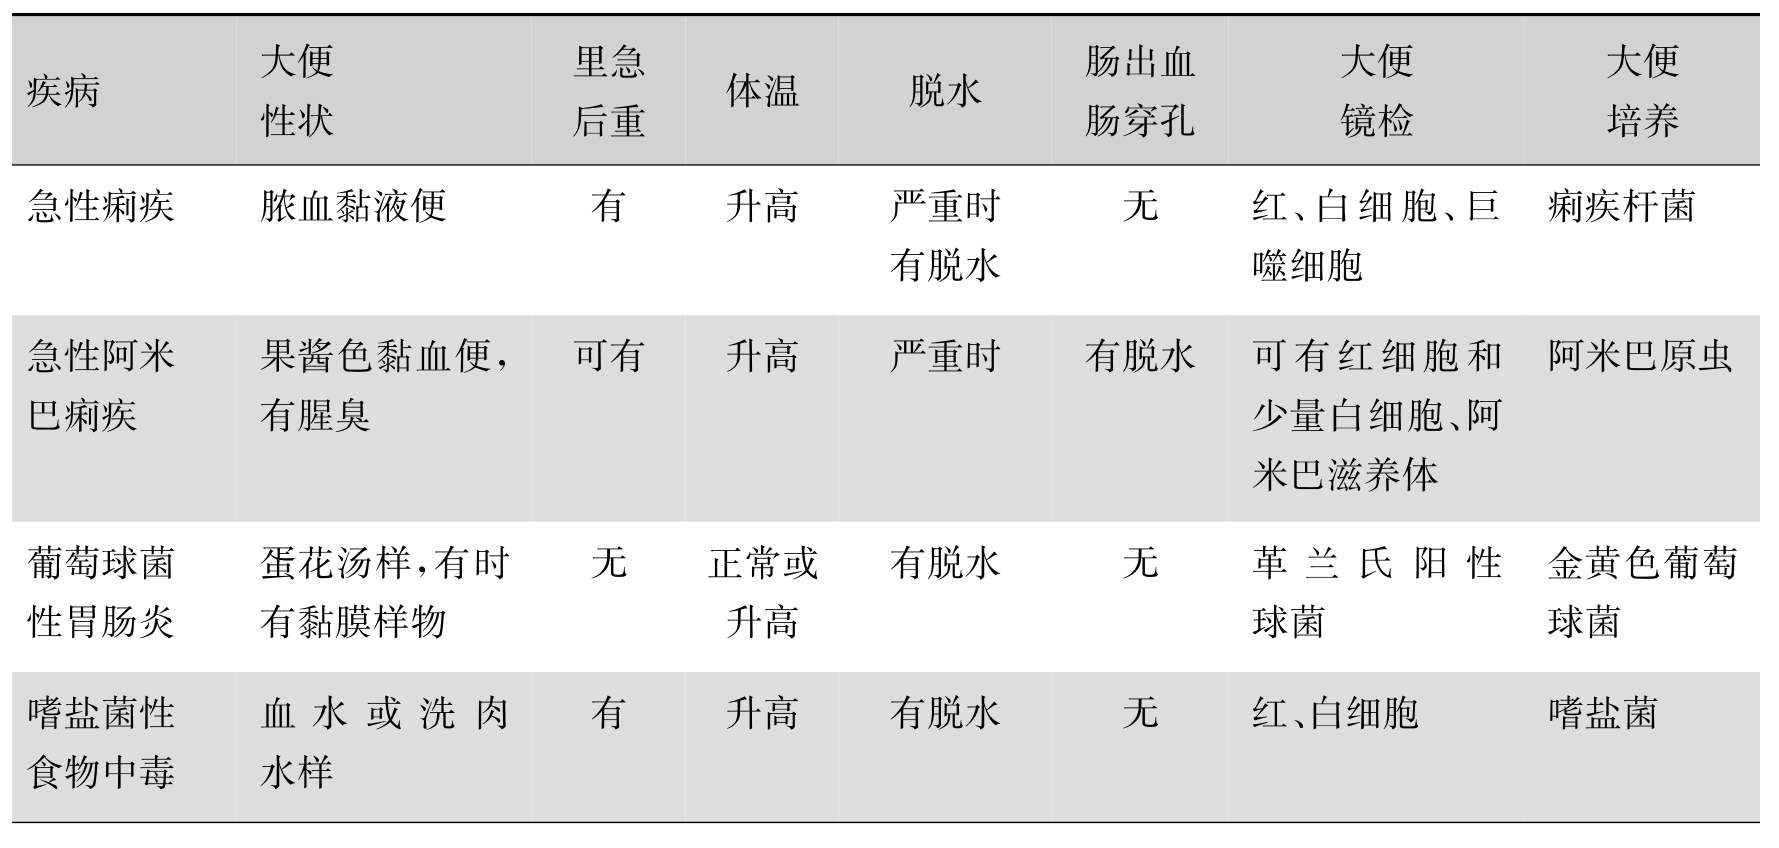
\includegraphics[width=\textwidth,height=\textheight,keepaspectratio]{./images/Image00131.jpg}\\
 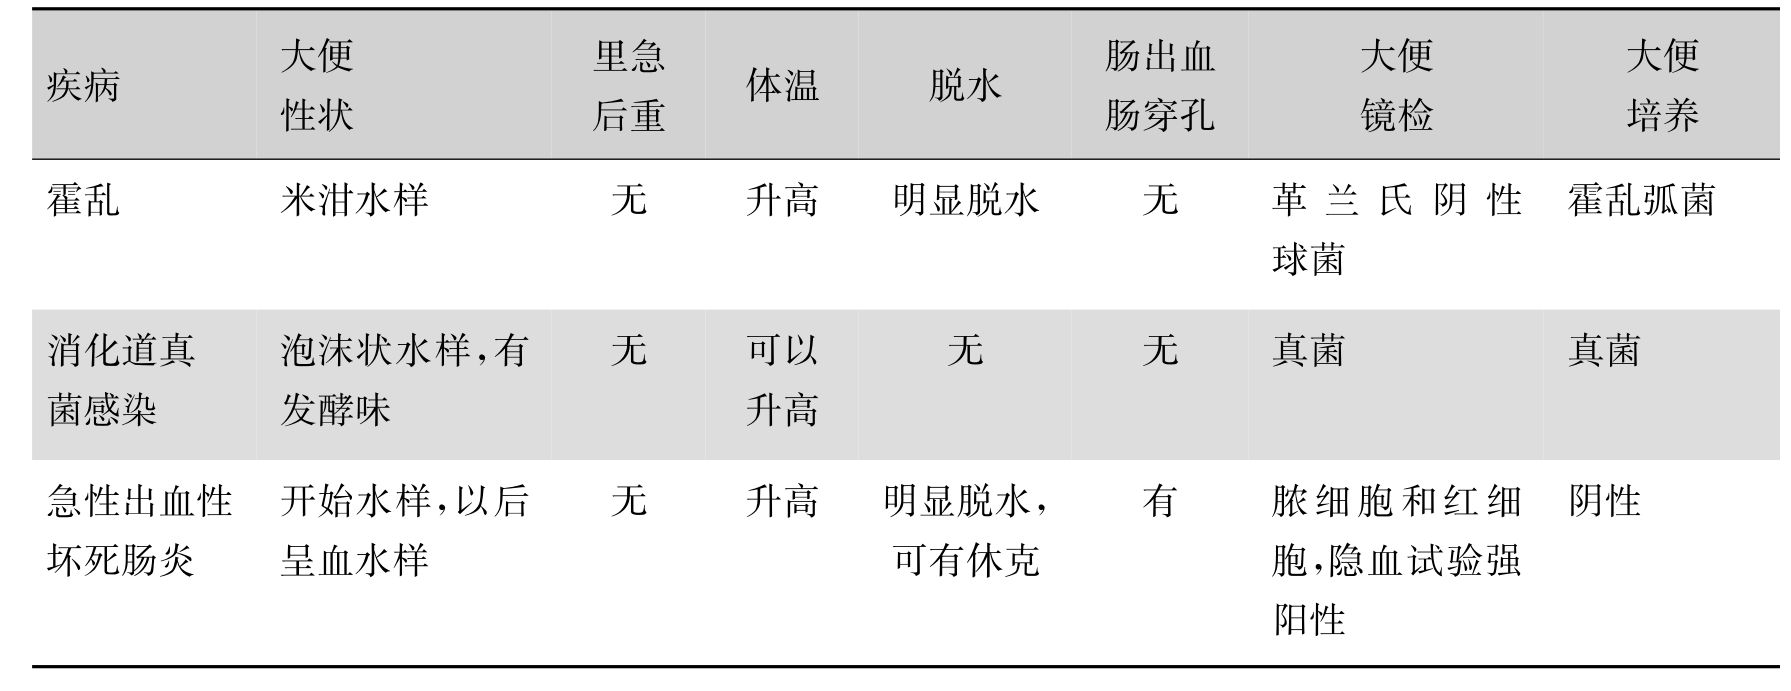
\includegraphics[width=\textwidth,height=\textheight,keepaspectratio]{./images/Image00132.jpg}
 \end{longtable}

\protect\hypertarget{text00188.html}{}{}

\section{参考文献}

1.刘思纯.肠道正常菌群及菌群失调.新医学,1999,30(11):626

2.符立龙,等.2001~2005年湛江市食物中毒情况分析.国际医药卫生导报,2007,13(15):164-167

3.毕水莲,李琳,唐书泽,等.变形杆菌属食物中毒的特点与防控措施.现代食品科技,2009(6):690-695

4.姜晓清,施永林.一起金黄色葡萄球菌引起的食物中毒调查.现代预防医学,2008,35(22):4354

5.蓝弘.两起肉毒杆菌食物中毒事件的分析.第三军医大学学报,2007,29(21):2106-2107

6.李晓艳,吕碧锋,潘海晖,等.529例副溶血弧菌食物中毒分析.现代医药卫生,2008,24(5):778

7.张翔,浦政轶.一起铜绿假单胞菌引起食物中毒的调查分析.交通医学,2002,16(5):465

8.王琼,邱羽,曾凡胜,等.深圳地区秋冬季婴幼儿病毒性腹泻病原分析.中华检验医学杂志,2009,32(8):873-876

9.钟豪杰,常昭瑞,张静,等.中国2007年细菌性痢疾监测分析.中华流行病学杂志,2010,31(3):304-307

10.胡瑞华,任红,张培林,等.霍乱的流行病学和分子流行病学.国际流行病学传染病学杂志,2006,33(4):268-270,274

11.于恩庶.中国小肠结肠炎耶尔森氏菌病研究进展.中华流行病学杂志,2000,21(6):453-455

12.陈杰,孙新婷,曾争,等.急性空肠弯曲菌肠炎的临床特征及耐药性分析.传染病信息,2011,24(1):21-22,25

13.王颖.危重症患者抗生素相关性腹泻的临床特点及危险因素分析.中国医师进修杂志,2010,33(31):71-72,75

14.杨建国,吴凤友.喹诺酮类药物治疗急性阿米巴痢疾临床分析.中华内科杂志,1991,30(9):569-571

15.祖述宪.隐孢子虫病研究现状.安徽医科大学学报,2000,35(2):83-88

16.杭德荣,黄轶昕,洪青标,等.2002~2007年江苏省急性血吸虫病疫情分析.中国血吸虫病防治杂志,2008,20(5):350-353

17.曹先.急性臭米面中毒四例.中华急诊医学杂志,2007,16(3):286-286

18.常见植物性食物中毒及急救措施.继续医学教育,2007,21(24):36-40

19.刘定华,冯东侠,江莲,等.急性河豚中毒患者脑氧供需平衡变化的临床研究.中华急诊医学杂志,2004,13(11):766-768

20.周晶,王海珍,陈灵敏,等.血液净化治疗急性鱼胆中毒致多器官功能衰竭7例临床分析.中华危重症医学杂志(电子版),2012,5(4):39-41

21.钟勇,杨世永,杨芳智,等.血液灌流联合血液透析抢救重度有机磷农药中毒62例.中国危重病急救医学,2011,23(4):212

22.杨维良,张东伟,张新晨,等.成人急性出血性坏死性小肠炎78例的诊断与手术治疗.中华胃肠外科杂志,2005,8(3):260-261

23.炎症性肠病诊断与治疗的共识意见(2012年,广州).胃肠病学,2012,17(12):763-781

24.曾德唯,张静.症状监测在伤寒和副伤寒防治中的应用.中华流行病学杂志,2010,31(9):1053-1055

25.高翔,胡品津,郑瑶,等.炎症性肠病患者血清中自身抗体检测的临床意义.中华内科杂志,2005,44(6):428-430

\protect\hypertarget{text00189.html}{}{}

